\chapter{Projeto - Parte 4}\label{ch:projeto-parte4}

TODO()


\section{Arquitetura Deliberativa}\label{sec:arquitetura-deliberativa}

Conforme foi abordado na secção~\ref{sec:arquiteturas-reativa-memoria}, um agente reativo com memória age com conhecimento do presente, através de reações a estímulos, e com conhecimento do passado, através da memorização de percepções e de ações passadas.
Um agente deliberativo, além de possuir as características de um agente reativo com memória, é capaz de antecipar o futuro, através da simulação de cenários, e consequentemente de planear ações futuras, com base em objetivos explícitos (fixos ou gerados dinamicamente) e em processos de deliberação sobre que objetivos concretizar e quais os meios a utilizar.

Qualquer sistema para poder antecipar o futuro tem que ter conhecimento (modelo do mundo), e esse conhecimento pode ser adquirido através da experiência ou de algo que já tenha esse conhecimento e o transmita para o agente (e.g., num ambiente multi-agente, um agente pode adquirir conhecimento de outro agente).
O modelo do mundo caracteriza-se como um caso particular da representação do modelo do problema, e permite simular para cada opção as múltiplas sequências de evolução possíveis, através de uma simulação interna~\cite{isel:iasa:slides:arq-agentes-deliberativos}.

A sequência de ações geradas por um agente deliberativo, através de processos internos, caracterizam o seu comportamento, ao contrário dos agentes reativos que têm comportamentos baseados em reações.

Numa arquitetura deliberativa, o módulo de memória é indispensável e dá suporte à simulação interna e aos mecanismos de deliberação~\cite{isel:iasa:slides:arq-agentes-deliberativos}, conforme representado na figura~\ref{fig:arquitetura-deliberativa}.

\begin{figure}[H]
    \begin{center}
        \resizebox{100mm}{!}{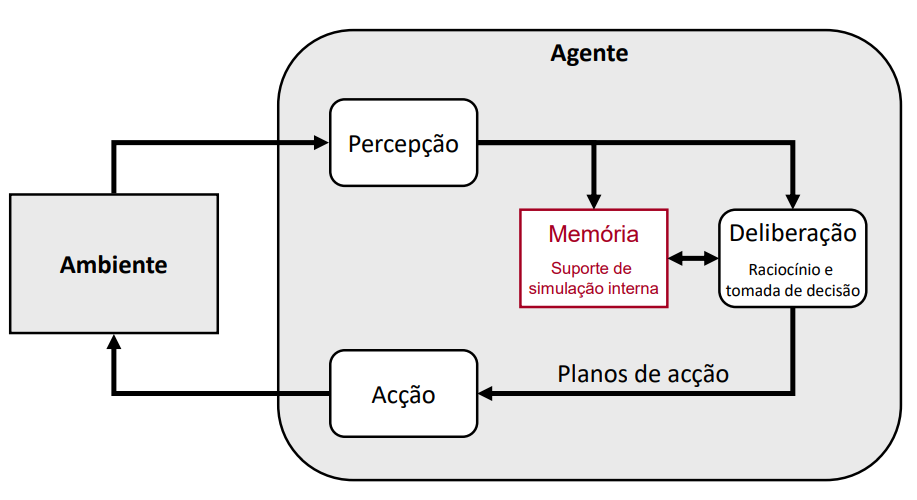
\includegraphics{../figures/arquitetura-deliberativa}}
    \end{center}
    \caption{Arquitetura deliberativa.
    Retirado de~\cite{isel:iasa:slides:arq-agentes-deliberativos}, slide 16.}
    \label{fig:arquitetura-deliberativa}
\end{figure}


\section{Raciocínio Automático}\label{sec:raciocinio-automatico-1}

Conforme foi abordado na secção~\ref{sec:raciocinio-automatico}, o raciocínio automático é um processo de inferência que permite a um agente deliberativo deduzir novas informações a partir de conhecimento prévio.

Com base nos conhecimentos adquiridos nesta fase do projeto, este raciocínio pode ser subdividido em dois tipos:

\begin{itemize}
    \item \textbf{Raciocínio Prático}: orientado para a ação (interação permanente com o mundo, ao qual está associado o processo de tomada de decisão).
    Tem como input os objetivos a atingir, as ações realizáveis e a representação do mundo, e como output os planos de ação.
    \item \textbf{Raciocínio Teórico}: orientado para o conhecimento, que permite deduzir novas informações a partir de conhecimento prévio.
    Caracteriza-se por ser direto, ou seja, não envolve interação com o mundo.
\end{itemize}

\subsection{Raciocínio Prático}\label{subsec:raciocinio-pratico}

Numa arquitectura deliberativa, o raciocínio prático suporta o processo
geral de tomada de decisão que determina o comportamento do agente,
ou seja, quais as acções a realizar perante as percepções obtidas e o
estado do modelo interno do mundo~\cite{isel:iasa:slides:arq-agentes-deliberativos}.
Este processo de tomada de decisão é composto por duas fases:

\begin{itemize}
    \item \textbf{Deliberação}: raciocínio sobre os fins, que permite definir os objetivos a atingir (i.e., opções (input) -> objetivos (output)).
    \item \textbf{Planeamento}: raciocínio sobre os meios, que permite definir os planos de ação a executar (i.e., ações (input) -> planos (output)).
\end{itemize}

Tendo em conta que o raciocínio prático é um processo de tomada de decisão, é necessário que o agente tenha objetivos, que são os critérios de avaliação das ações, e que possa avaliar as ações possíveis, de forma a escolher a melhor ação a executar.
Portanto, a deliberação sobre a representação do modelo do mundo que permite definir os objetivos, e o planeamento com base nesses e nos meios disponíveis, definem os processos necessários para a geração de planos de ação, conforme representado na figura~\ref{fig:delib-planeamento}.

\begin{figure}[H]
    \begin{center}
        \resizebox{100mm}{!}{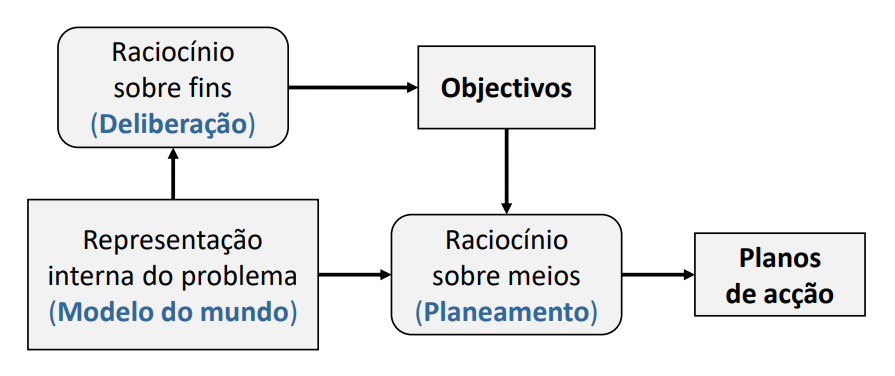
\includegraphics{../figures/delib-planeamento}}
    \end{center}
    \caption{Deliberação e planeamento num agente deliberativo.
    Retirado de~\cite{isel:iasa:slides:arq-agentes-deliberativos}, slide 8.}
    \label{fig:delib-planeamento}
\end{figure}

No entanto, o ambiente pode ser dinâmico, e por isso o agente pode ter que reagir a mudanças no ambiente (i.e., alterações no modelo do mundo), o que implica que o processo de tomada de decisão seja adaptativo, ou seja, que possa ser reavaliado e ajustado (reconsideração).
Além disso, mesmo sem alteração do estado do ambiente, o próprio plano de ação pode alterar-se ao longo do tempo e estar desfasado da realidade, devido a um acontecimento que não foi antecipado (e.g., um camião que seguia um trajeto específico, mas por causa de areia no caminho, teve que mudar de trajeto).

Portanto, o processo geral de tomada de decisão, que ocorre de forma cíclica, pode ser então representado pelos seguintes passos~\cite{isel:iasa:slides:arq-agentes-deliberativos}:

\begin{enumerate}
    \item Observar o mundo, gerando percepções.
    \item Atualizar o modelo do mundo, com base nas percepções.
    \item Se reconsiderar, então:
    \begin{enumerate}
        \item Deliberar o que fazer, gerando um conjunto de objetivos.
        \item Planear como fazer, gerando um plano de ação.
    \end{enumerate}
    \item Executar o plano de ação.
\end{enumerate}

\subsection{Racionalidade Limitada}\label{subsec:racionalidade-limitada}

A racionalidade limitada é um conceito que se aplica a agentes que têm recursos computacionais limitados (i.e., tempo de computação, memória), e que por isso não conseguem gerar planos de ação ótimos.

Um agente com racionalidade limitada tenta chegar a uma solução satisfatória, não à melhor solução, de forma dinâmica, tendo em conta os recursos computacionais disponíveis.
Divide o problema em subproblemas mais simples, aplicando restricções de forma a reduzir a complexidade do problema, e resolve-os sequencialmente, de forma a atingir o objetivo final~\cite{isel:iasa:slides:arq-agentes-deliberativos}.

Para o contexto humano, não é possível fazer raciocínio ótimo mas sim automático, devido à racionalidade limitada.


\section{Planeamento Automático}\label{sec:planeamento-automatico}

O planeamento automático é um processo deliberativo, que faz parte do raciocínio prático,
que tem por objetivo
gerar sequências de ação, designadas planos~\cite{isel:iasa:slides:plan-autom-pee}.
Um processo de planeamento requer um modelo de planeamento que define a representação abstrata do problema a resolver, e que apresenta os mesmos conceitos que foram abordados na secção~\ref{subsec:modelacao-problema} (i.e., estados, operadores, etc...).
Dado um modelo de planeamento e um conjunto de objetivos provenientes do processo de deliberação, o planeador gera um plano de ação que permite ao agente concretizar esses objetivos.

Este processo é realizado através de métodos de raciocínio automático, como a procura em
espaço de estados e a procura por processos de decisão de Markov~\cite{isel:iasa:slides:plan-autom-pee}.

\subsection{Planeador Baseado em PEE}\label{subsec:planeador-baseado-em-pee}

No caso de um planeador baseado em procura em espaços de estados (PEE), é necessário considerar~\cite{isel:iasa:slides:plan-autom-pee}:

\begin{itemize}
    \item Modelo do problema de planeamento.
    \item Heurística a utilizar (se necessário) para guiar a procura (ver secção~\ref{subsubsec:heuristica}).
    \item Mecanismo de procura (ver secção~\ref{sec:mecanismo-procura}).
\end{itemize}

\subsection{Planeador Baseado em PDM}\label{subsec:planeador-baseado-em-pdm}

No caso de um planeador baseado em processos de decisão de Markov (PDM), a representação do domínio do problema é feita sobre a forma de um processo de decisão de Markov, que se define como um modelo matemático que descreve um sistema que evolui ao longo do tempo, com base em estados e ações, e que é utilizado para modelar situações de decisão sequencial sob incerteza~\cite{isel:iasa:slides:plan-autom-pdm}.

Ao contrário do planeador baseado em PEE, o planeador baseado em PDM não gera um plano de ação, mas sim uma política.
Esta política define-se como uma função que mapeia estados em ações, e que é utilizada para determinar a ação a executar em cada estado, definindo a estratégia de tomada de decisão do agente.

Além disso, em vez de só ter em conta o custo, o planeador baseado em PDM tem em conta a utilidade de uma ação que depende de uma sequência de decisões, da possibilidade de ganhos e perdas, da incerteza na decisão e do efeito cumulativo~\cite{isel:iasa:slides:processos-decisao-sequencial}.


\section{Processos de Decisão Sequencial}\label{sec:processos-de-decisao-sequencial}

No processo de decisão geral, cada estado $s$ é caracterizado por um conjunto de atributos que descrevem o estado do mundo, e cada ação $a$ é uma transformação que altera o estado do mundo, levando a um novo estado $s'$~\cite{isel:iasa:slides:processos-decisao-sequencial}.
O valor (utilidade) desses estados e decisões pode não ser conhecido de imediato, sendo percebido apenas de forma diferida no tempo, devido a potenciais encadeamentos de estados e possíveis decisões futuras, conforme representado na figura~\ref{fig:processo-decisao-sequencial}.

No processo de decisão sequencial, a evolução entre estados ocorre por efeito de ações que, no caso geral, podem ser não deterministas, ou seja, o resultado das ações pode não ser completamente previsível, podendo existir incerteza no seu resultado.
Esse tipo de processos corresponde a espaços de estados (ambientes) não deterministas (estocásticos), nos quais as transições entre estados ocorrem por efeito das ações, cada uma com uma probabilidade associada de forma a representar a incerteza do ambiente. A cada transição pode estar associada uma recompensa, que representa o ganho ou perda relacionado a essa transição de estado~\cite{isel:iasa:slides:processos-decisao-sequencial}.

\begin{figure}[H]
    \begin{center}
        \resizebox{100mm}{!}{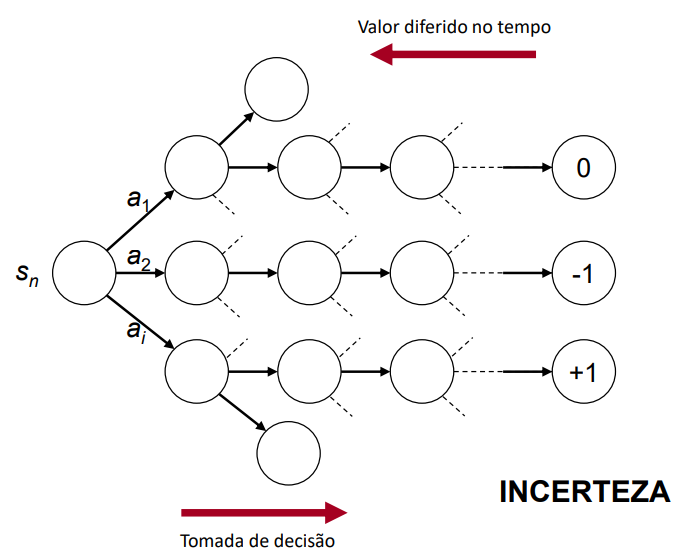
\includegraphics{../figures/processo-decisao-sequencial}}
    \end{center}
    \caption{Processo de decisão sequencial.
    Retirado de~\cite{isel:iasa:slides:processos-decisao-sequencial}, slide 3.}
    \label{fig:processo-decisao-sequencial}
\end{figure}


\section{Cadeias de Markov}\label{sec:cadeias-de-markov}

Uma cadeia de Markov~\cite{wiki:markov-chain} é um processo estocástico que evolui ao longo do tempo, com
base em estados e transições entre esses estados, e que obedece à propriedade de Markov~\cite{isel:iasa:slides:processos-decisao-sequencial}.

A propriedade de Markov é uma propriedade em processos estocásticos, que se caracteriza pela distribuição probabilística condicional dos estados futuros de um processo depender exclusivamente do estado presente (i.e., a previsão dos estados seguintes só depende do estado presente)~\cite{isel:iasa:slides:processos-decisao-sequencial}.

Formalmente, uma cadeia de Markov é definida por um conjunto de estados $S$ e por uma função de transição $T$, que define a probabilidade de transição de um estado para outro,
conforme representado na figura~\ref{fig:cadeia-de-markov}.

\begin{figure}[H]
    \begin{center}
        \resizebox{100mm}{!}{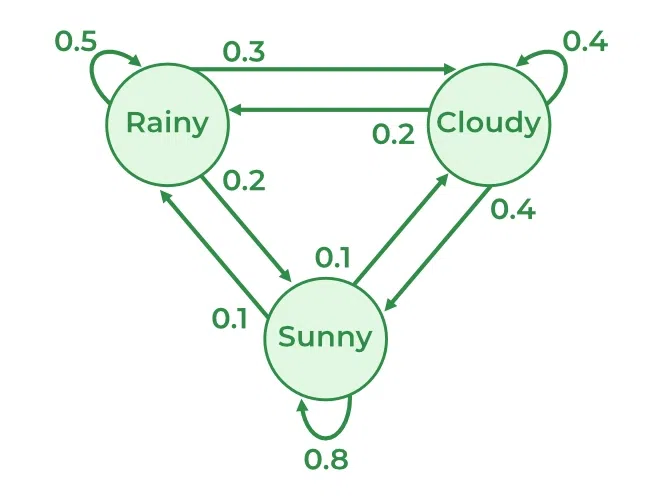
\includegraphics{../figures/cadeia-markov}}
    \end{center}
    \caption{Cadeia de Markov.
    Retirado de~\cite{isel:iasa:slides:processos-decisao-sequencial}, slide 7.}
    \label{fig:cadeia-de-markov}
\end{figure}


\section{Processos de Decisão de Markov}\label{sec:processos-de-decisao-de-markov}

O processo de decisão de Markov (PDM) é um processo de controlo estocástico em tempo discreto, e que fornece um modelo matemático para modelar situações de decisão sequencial sob incerteza~\cite{wiki:markov-decision-process}.
Esta incerteza resulta da impossibilidade de se obter informação completa relativa ao domínio do problema (e.g., navegação em veículos autónomos).
Este processo caracteriza-se como uma extensão de uma cadeia de Markov, que inclui, além dos estados e transições; ações e recompensas, de forma a obter uma política.
Formalmente, é representado pelo seguinte conjunto de elementos:

\begin{itemize}
    \item \textbf{$S$}: conjunto finito de estados;
    \item \textbf{Modelo de transição}: \( T(s, a, s') \), onde \( s \) é o estado atual, \( a \) é a ação a ser tomada, e \( s' \) é o estado futuro.
    é a probabilidade de mudança de estado de \( s \) para \( s' \) após a ação \( a \) ser tomada.
    Em ambientes deterministas, a probabilidade de transição é 1, e em ambientes estocásticos, a probabilidade de transição é um valor entre 0 e 1;
    \item \textbf{Modelo de recompensa}: \( R(s, a, s') \), onde \( s \) é o estado atual, \( a \) é a ação a ser tomada, e \( s' \) é o estado futuro.
    é a recompensa associada à transição de estado de \( s \) para \( s' \) após a ação \( a \) ser tomada.
    Este modelo está descrito no caso geral, mas poderá estar dependente apenas do estado atual e da ação tomada ou apenas do estado atual;
    \item \textbf{Factor de desconto}: \( \gamma \), onde \( 0 \leq \gamma \leq 1 \), que é o fator de retenção aplicado à recompensa.
    Por cada unidade de tempo que passa, a recompensa é descontada por um fator de \( \gamma \), de forma exponencial.
    Se \( \gamma = 0 \), a tomada de decisão só depende do presente, porque o futuro é anulado.
\end{itemize}

\subsection{Utilidade}\label{subsec:utilidade}

O valor (utilidade) de um estado caracteriza-se com o efeito acumulativo que vai tendo do mundo, através dos ganhos e perdas que vai obtendo, diferidos no tempo, visto que pode existir perda de oportunidade na passagem do tempo (e.g., no mercado financeiro, o valor de uma ação é volátil e varia ao longo do tempo).
No entanto, poderão existir estados em que não existem ganhos e perdas.

Portanto, a utilidade representa o valor de se estar num estado, para efeito de concretização de um objetivo do sistema, mas representa o valor a longo prazo (na história de evolução do sistema) (e.g., um automóvel pode ter que acelarar, gastando mais combustivel, para evitar um acidente, mas a longo prazo, o valor de evitar o acidente é maior do que o valor de gastar mais combustivel).

\subsection{Política}\label{subsec:politica-otima}

Uma política ($\pi$) é uma função que mapeia estados em ações, e que é utilizada para determinar a ação a executar em cada estado, definindo a estratégia de tomada de decisão do agente.
É caracterizada em dois tipos:

\begin{itemize}
    \item \textbf{Determinística}: mapeia cada estado em apenas uma ação ($\pi : S \rightarrow A(s); \quad s \in S$);
    \item \textbf{Estocástica}: mapeia cada estado numa distribuição de probabilidade sobre as ações possíveis ($\pi : S \times A(s) \rightarrow [0,1]; \quad s \in S$).
\end{itemize}

\subsection{Objetivo}\label{subsec:objetivo}

O objetivo de um processo de decisão de Markov é determinar a política ótima ($\pi^*$), que é a política que maximiza a utilidade esperada, ou seja, a política que maximiza a recompensa esperada ao longo do tempo, através das equações de Bellman~\cite{wiki:bellman-equation}.
Devido à propriedade de Markov, a utilidade de um estado dada uma ação é a soma da recompensa imediata e da utilidade esperada do estado seguinte, ponderada pelo fator de desconto $\gamma$, conforme representado na equação de Bellman~\ref{eq:bellman-utilidade-acao}.

\begin{equation}
    \label{eq:bellman-utilidade-acao}
    U(s, a) = \sum_{s'} T(s, a, s') [R(s, a, s') + \gamma U^\pi(s')]
\end{equation}

De forma a calcular a utilidade esperada de um estado, é necessário considerar a ação que maximiza a utilidade esperada desse estado, conforme representado na equação de Bellman~\ref{eq:bellman-utilidade-final}.

\begin{equation}
    \label{eq:bellman-utilidade-final}
    Ufinal(s) = \max_{a} U(s, a)
\end{equation}

A partir da utilidade esperada de cada estado, é possível determinar a política ótima ($\pi^*$), que é a política que seleciona a ação que maximiza a utilidade esperada de cada estado, conforme representado na equação de Bellman~\ref{eq:bellman-politica-otima}.

\begin{equation}
    \label{eq:bellman-politica-otima}
    \pi^*(s) = \arg\max_{a} Ufinal(s, a)
\end{equation}

\subsubsection{Algoritmo de Iteração de Valor}\label{subsubsec:algoritmo-iteracao-valor}

O algoritmo de iteração de valor é um algoritmo que permite calcular a utilidade ótima de cada estado, através da iteração de cálculos de utilidade, até que a utilidade de cada estado convirja para um valor estável.
Este algoritmo inicializa a utilidade de cada estado a zero e, de forma iterativa, calcula a utilidade de cada estado, conforme a equação de Bellman~\ref{eq:bellman-utilidade-acao}, até que um determinado critério de convergência seja atingido~\cite{isel:iasa:slides:processos-decisao-sequencial}.

O critério de convergência é representado por um $\delta$, que define a diferença máxima permitida entre a utilidade atual de um estado e a utilidade do estado na iteração anterior.
À medida que as utilidades de cada estado são atualizadas ao longo das iterações, elas convergem para valores muito próximos, até que a partir de um determinado ponto são consideradas irrizórias, e consequentemente consideradas estáveis.

O algoritmo apresenta assim 2 ciclos: um ciclo externo que controla a convergência do algoritmo, e um ciclo interno que calcula a utilidade para cada estado, conforme ilustrado na figura~\ref{fig:algoritmo-iteracao-valor}.

\begin{figure}[H]
    \begin{center}
        \resizebox{100mm}{!}{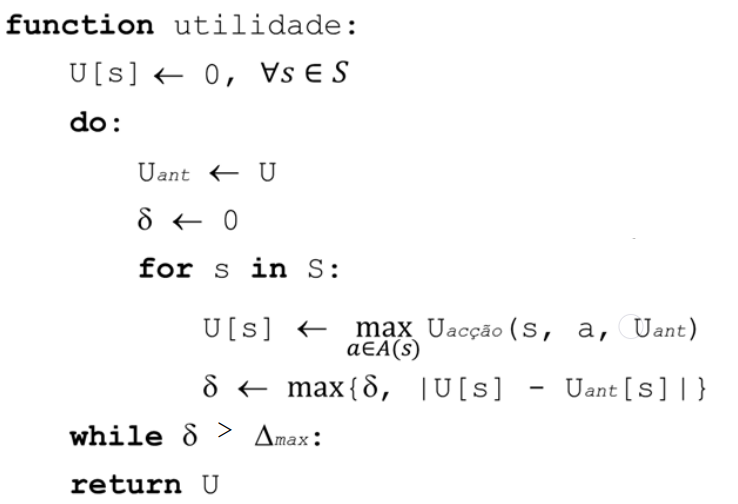
\includegraphics{../figures/algoritmo-iter-valor}}
    \end{center}
    \caption{Algoritmo de iteração de valor.
    Retirado de~\cite{isel:iasa:slides:processos-decisao-sequencial}, slide 21.}
    \label{fig:algoritmo-iteracao-valor}
\end{figure}

\section{Aprendizagem por Reforço}\label{sec:aprendizagem-por-reforco}

TODO()

\section{Implementação do Agente Deliberativo com PEE}\label{sec:implementacao-agente-deliberativo-com-pee}
TODO()


\section{Implementação do Agente Deliberativo com PDM}\label{sec:implementacao-agente-deliberativo-com-pdm}
TODO()
